\documentclass[11pt]{article}

\usepackage{tikz}
\usepackage{pgf}
\usepackage{amsmath}
\usepackage{physics}
\usepackage[offset=1.2em]{simpler-wick}

\usetikzlibrary{arrows}
\usetikzlibrary{shapes.misc}

\tikzset{cross/.style={cross out, draw=black, fill=none, minimum size=2*(#1-\pgflinewidth), inner sep=0pt, outer sep=0pt}, cross/.default={2pt}}

% Arrow in the middle
\usetikzlibrary{decorations.markings}
%\newcommand{\midarrow}{\tikz \draw[-triangle 90] (0,0) -- +(.1,0);}

\title{Drawings That We Use in Many-Body Physics}
\author{Greg Winther}
\date{\today}

\begin{document}

	\maketitle

	\section{Slater determinants}
	
	Drawing the reference state will result in a drawing of nothing. A single-excited reference
	state is two vertical arrows
	
	\begin{align}	
		\Phi_i^a =
		\begin{tikzpicture}[baseline=0]
		\begin{scope}[decoration={markings, mark=at position 0.52 with {\arrow{>}}}]
			\draw[postaction={decorate}] (1, -1) --  (1, 1) node [anchor=east,pos=0.5] {i};
			\draw[postaction={decorate}](1.5, 1) -- (1.5, -1) node [anchor=west,pos=0.5] {a};
		\end{scope}
		\end{tikzpicture},
	\end{align}
	
	while the double-excited Slater determinant consists of four vertical arrows,
	
	\begin{align}	
		\Phi_{ij}^{ab} =
		\begin{tikzpicture}[baseline=0]
		\begin{scope}[decoration={markings, mark=at position 0.52 with {\arrow{>}}}]
			\draw[postaction={decorate}] (1, -1) --  (1, 1) node [anchor=east,pos=0.5] {i};
			\draw[postaction={decorate}](1.5, 1) -- (1.5, -1) node [anchor=west,pos=0.5] {a};
			\draw[postaction={decorate}] (2.5, -1) --  (2.5, 1) node [anchor=east,pos=0.5] {j};
			\draw[postaction={decorate}](3, 1) -- (3, -1) node [anchor=west,pos=0.5] {b};
		\end{scope}
		\end{tikzpicture}.
	\end{align}
	
	The horizontal positions of the lines have no significance. If we want to indicate a bra or ket form 
	we draw a couple of horizontal lines,
	
	\begin{align}
		\ket{\Phi_i^a} = \{ \hat{a}^\dagger \hat i\} \ket{0} = 
		\begin{tikzpicture}[baseline=0]
		\begin{scope}[decoration={markings, mark=at position 0.52 with {\arrow{>}}}]
			\draw[postaction={decorate}] (1, -1) --  (1, 1) node [anchor=east,pos=0.5] {i};
			\draw[postaction={decorate}](1.5, 1) -- (1.5, -1) node [anchor=west,pos=0.5] {a};
			\draw(0.75, -1) -- (1.75, -1);
			\draw(0.75, -1.1) -- (1.75, -1.1);
		\end{scope}
		\end{tikzpicture}, \quad
		\bra{\Phi_i^a} = \bra{0} \{ \hat{i}^\dagger \hat a\} = 
		\begin{tikzpicture}[baseline=0]
		\begin{scope}[decoration={markings, mark=at position 0.52 with {\arrow{>}}}]
			\draw[postaction={decorate}] (1, -1) --  (1, 1) node [anchor=east,pos=0.5] {i};
			\draw[postaction={decorate}](1.5, 1) -- (1.5, -1) node [anchor=west,pos=0.5] {a};
			\draw(0.75, 1) -- (1.75, 1);
			\draw(0.75, 1.1) -- (1.75, 1.1);
		\end{scope}
		\end{tikzpicture},
	\end{align}
	
	where  $\{ABC\dots\}$ is a normal ordered product relative to the Fermi vacuum.
	A double-excited ket state could be drawn like
	
	\begin{align}
		\ket{\phi_{ij}^{ab}} = \{\hat{a}^\dagger \hat{b}^\dagger \hat{j} \hat{i} \} \ket{0}
			= \{ (\hat{a}^\dagger \hat{i}) (\hat{b}^\dagger \hat{j})\} \ket{0} =
			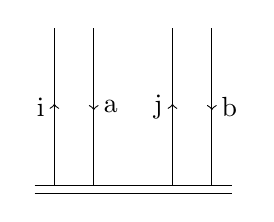
\begin{tikzpicture}[baseline=0]
			\begin{scope}[decoration={markings, mark=at position 0.52 with {\arrow{>}}}]
				\draw[postaction={decorate}] (1, -1) --  (1, 1) node [anchor=east,pos=0.5] {i};
				\draw[postaction={decorate}](1.5, 1) -- (1.5, -1) node [anchor=west,pos=0.5] {a};
				\draw[postaction={decorate}](2.5, -1) -- (2.5, 1) node [anchor=east,pos=0.5] {j};
				\draw[postaction={decorate}](3, 1) -- (3, -1) node [anchor=west,pos=0.5] {b};				
				\draw(0.75, -1) -- (3.25, -1);
				\draw(0.75, -1.1) -- (3.25, -1.1);
			\end{scope}
			\end{tikzpicture}
	\end{align}
	
	This drawing could, however, also mean $\ket{\phi_{ij}^{ba}}$. The use of diagrams will 
	be independent of this ambiguity, as long as one remains consistent. To be precise one can
	introduce dotted/dashed lines,
	
	\begin{align}
		\ket{\phi_{ij}^{ab}} = \{\hat{a}^\dagger \hat{b}^\dagger \hat{j} \hat{i} \} \ket{0}
			= \{ (\hat{a}^\dagger \hat{i}) (\hat{b}^\dagger \hat{j})\} \ket{0} =
			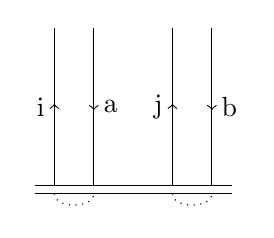
\begin{tikzpicture}[baseline=0]
			\begin{scope}[decoration={markings, mark=at position 0.52 with {\arrow{>}}}]
				\draw[postaction={decorate}] (1, -1) --  (1, 1) node [anchor=east,pos=0.5] {i};
				\draw[postaction={decorate}](1.5, 1) -- (1.5, -1) node [anchor=west,pos=0.5] {a};
				\draw[dotted](1, -1.1) to[out=-90,in=-90] (1.5,-1.1);				
				\draw[postaction={decorate}](2.5, -1) -- (2.5, 1) node [anchor=east,pos=0.5] {j};
				\draw[postaction={decorate}](3, 1) -- (3, -1) node [anchor=west,pos=0.5] {b};
				\draw[dotted](2.5, -1.1) to[out=-90,in=-90] (3,-1.1);			
				\draw(0.75, -1) -- (3.25, -1);
				\draw(0.75, -1.1) -- (3.25, -1.1);
			\end{scope}
			\end{tikzpicture}.
	\end{align}
	
	These indicate what index letters should be above and below one another.
	
	\section{One-Particle Operators}
	
	The one-electron operator on normal-ordered from is given by
	
	\begin{equation}
		\hat{U}_N = \sum_{pq} \bra{p} \hat{u} \ket{q} \{\hat{p}^\dagger \hat{q} \},
	\end{equation}
	
	acting on a singly excited Slater determinant
	
	\begin{equation}
		\ket{\Phi^a_i} = \{ \hat{a}^\dagger \hat{i} \}\ket{0},
	\end{equation}
	
	id est
	
	\begin{equation}
		\sum_{pq} \bra{p} \hat{u} \ket{q} \{\hat{p}^\dagger \hat{q} \}\{ \hat{a}^\dagger \hat{i} \}\ket{0}.
	\end{equation}
	
	There are four different terms arising from this expression, depending on whether $p$ and $q$
	represents particles or holes. Beginning with a \emph{particle}-\emph{particle} term,
	
	\begin{equation}
		\begin{aligned}
			\bra{b} \hat{u} \ket{c} \{ \hat{b}^\dagger \hat{c} \} \{ \hat{a}^\dagger \hat{i} \} \ket{0} 
				&= \bra{b} \hat{u} \ket{c} \{ \hat{b}^\dagger \hat{c} \hat{a}^\dagger \hat{i} \} \ket{0}
				+	   \bra{b} \hat{u} \ket{c} \{\wick{  \hat{b}^\dagger  \c{\hat{c}}  \c{\hat{a}}^\dagger \hat{i} } \} \ket{0}\\
				&= \bra{b} \hat{u} \ket{c} \hat{b}^\dagger\hat{a}^\dagger\hat{i}\hat{c}\ket{0}
				+	  \bra{b} \hat{u} \ket{c} \delta_{ac}\{\hat{b}^\dagger \hat{i} \} \\
				&= 0 + \bra{b} \hat{u} \ket{c} \delta_{ac}\ket{\Phi_i^a},
		\end{aligned}
	\end{equation}
	
	giving non-zero contributions of the type
	\begin{equation}
		\bra{b} \hat{u} \ket{a} \{ \hat{b}^\dagger \hat{a} \} \ket{\Phi_i^a} 
			= \bra{b} \hat{u} \ket{a} \lvert \Phi_i^b \rangle.
	\end{equation}
	
	We can draw a graphical representation of this contraction process,
	
	\begin{equation}
		\begin{split}
			\begin{aligned}
			\bra{b}\hat{u}\ket{c} \{\hat{b}^\dagger \hat{c} \} &:\  
				\begin{tikzpicture}[baseline=0]
					\begin{scope}[decoration={markings, mark=at position 0.52 with {\arrow{>}}}]
						\draw (-1.2, 0)node[cross=4pt]{};
						\draw[dashed] (-1, 0) -- (0, 0);
						\draw[postaction={decorate}] (0, 0) -- (0.5, 1) node [anchor=west, pos=0.5]{b};
						\draw[postaction={decorate}] (0.5, -1) -- (0, 0) node [anchor=west, pos=0.5]{c}; 
					\end{scope}
				\end{tikzpicture}
			\\
			\ket{\Phi_i^a} &:\quad
				\begin{tikzpicture}[baseline=0]
					\begin{scope}[decoration={markings, mark=at position 0.52 with {\arrow{>}}}]
						\draw[postaction={decorate}] (1, -1) --  (1, 1) node [anchor=east,pos=0.5] {i};
						\draw[postaction={decorate}](1.5, 1) -- (1.5, -1) node [anchor=west,pos=0.5] {a};
						\draw(0.75, -1) -- (1.75, -1);
						\draw(0.75, -1.1) -- (1.75, -1.1);
				\end{scope}
			\end{tikzpicture}
		\end{aligned}
		\end{split} \ \to
		\begin{split}
				\begin{tikzpicture}
					\begin{scope}[decoration={markings, mark=at position 0.52 with {\arrow{>}}}]
						\draw (-1.2, 0)node[cross=4pt]{};
						\draw[dashed] (-1, 0) -- (0, 0);
						\draw[postaction={decorate}] (0, 0) -- (0.5, 1) node [anchor=west, pos=0.5]{b};
						\draw[postaction={decorate}] (0.5, -1) -- (0, 0) node [anchor=west, pos=0.5]{c}; 
						\draw[dotted] (0.5, -1) -- (0.5, -1.5) node[anchor=west, pos=0.5]
							{$\delta_{ac}$};
						\draw[postaction={decorate}] (0.5, -3.2) -- (0.5, -1.5) node [anchor=east,pos=0.5] {a};
						\draw[postaction={decorate}] (1, -1.5) -- (1, -3.2) node [anchor=west,pos=0.5] {i};
						\draw(0.25, -3.2) -- (1.25, -3.2);
						\draw(0.25, -3.3) -- (1.25, -3.3);
					\end{scope}
				\end{tikzpicture}
		\end{split} \to
		\begin{split}
			\begin{tikzpicture}
				\begin{scope}[decoration={markings, mark=at position 0.52 with {\arrow{>}}}]
					\draw[postaction={decorate}] (0.5, -1.1) -- (0.5, 1) node [anchor=east,pos=0.5] {b};
					\draw (-0.9, -1.1) node[cross=4pt]{};
					\draw[dashed] (-0.7, -1.1) -- (0.5, -1.1);
					\draw (0.5, -1.1) node[circle,fill,inner sep=1pt]{};
					\draw[postaction={decorate}] (0.5, -3.2) -- (0.5, -1.1) node [anchor=east,pos=0.5] {a};
					\draw[postaction={decorate}] (1, 1) -- (1, -3.2) node [anchor=west,pos=0.5] {i};
					\draw(0.25, -3.2) -- (1.25, -3.2);
					\draw(0.25, -3.3) -- (1.25, -3.3);
				\end{scope}
				\end{tikzpicture}
		\end{split}
	\end{equation}
	
	Now, let's consider a \emph{hole}-\emph{hole} term acting on the same single-excited Slater determinant,
	
	\begin{equation}
		\begin{aligned}
		\bra{j} \hat{u} \ket{k}\{ \hat{j}^\dagger \hat{k} \} \{ \hat{a}^\dagger \hat{i} \} \ket{0}
			&= \bra{j} \hat{u} \ket{k} \{ \hat{j}^\dagger \hat{k} \hat{a}^\dagger \hat{i} \} \ket{0}
			+   \bra{j} \hat{u} \ket{k} \{\wick{ \c{\hat{j}}^\dagger \hat{k} \hat{a}^\dagger \c{\hat{i}} } \} \ket{0} \\
			&= -\bra{j} \hat{u} \ket{k} \{ \hat{k} \hat{a}^\dagger \hat{i} \hat{j}^\dagger \} \ket{0}
			+     \delta_{ij}\bra{i} \hat{u} \ket{k} \{\hat{k} \hat{a}^\dagger \} \ket{0} \\
			&= 0 - \delta_{ij}\bra{i} \hat{u} \ket{j}\{ \hat{a}^\dagger \hat{k} \} \ket{0} \\
			&= - \delta_{ij} \bra{i} \hat{u} \ket{j} \ket{\Phi_k^a},
		\end{aligned}
	\end{equation}
	
	meaning we are only left with non-zero contributions of the type,
	
	\begin{equation}
		\bra{i} \hat{u} \ket{j}\{ \hat{i}^\dagger \hat{k} \} \ket{\Phi_i^a} = - \bra{i}\hat{u}\ket{k} \ket{\Phi_k^a}.
	\end{equation}

	One can make a diagrammatic representation of this contraction as well,
	
	\begin{equation}
		\begin{split}
			\begin{aligned}
			\bra{b}\hat{u}\ket{c} \{\hat{b}^\dagger \hat{c} \} &:\  
				\begin{tikzpicture}[baseline=0]
					\begin{scope}[decoration={markings, mark=at position 0.52 with {\arrow{>}}}]
						\draw (-1.2, 0)node[cross=4pt]{};
						\draw[dashed] (-1, 0) -- (0, 0);
						\draw[postaction={decorate}] (0.5, 1) -- (0, 0) node [anchor=west, pos=0.5]{k};
						\draw[postaction={decorate}] (0, 0) -- (0.5, -1) node [anchor=west, pos=0.5]{j}; 
					\end{scope}
				\end{tikzpicture}
			\\
			\ket{\Phi_i^a} &:\quad
				\begin{tikzpicture}[baseline=0]
					\begin{scope}[decoration={markings, mark=at position 0.52 with {\arrow{>}}}]
						\draw[postaction={decorate}] (1, -1) --  (1, 1) node [anchor=east,pos=0.5] {i};
						\draw[postaction={decorate}](1.5, 1) -- (1.5, -1) node [anchor=west,pos=0.5] {a};
						\draw(0.75, -1) -- (1.75, -1);
						\draw(0.75, -1.1) -- (1.75, -1.1);
				\end{scope}
			\end{tikzpicture}
		\end{aligned}
		\end{split} \ \to
		\begin{split}
				\begin{tikzpicture}
					\begin{scope}[decoration={markings, mark=at position 0.52 with {\arrow{>}}}]
						\draw (-1.2, 0)node[cross=4pt]{};
						\draw[dashed] (-1, 0) -- (0, 0);
						\draw[postaction={decorate}] (0.5, 1) -- (0, 0) node [anchor=west, pos=0.5]{k};
						\draw[postaction={decorate}] (0, 0) -- (0.5, -1) node [anchor=west, pos=0.5]{j}; 
						\draw[dotted] (0.5, -1) -- (0.5, -1.5) node[anchor=west, pos=0.5]
							{$\delta_{ij}$};
						\draw[postaction={decorate}] (1, -3.2) -- (1, -1.5) node [anchor=west,pos=0.5] {a};
						\draw[postaction={decorate}] (0.5, -1.5) -- (0.5, -3.2) node [anchor=east,pos=0.5] {i};
						\draw(0.25, -3.2) -- (1.25, -3.2);
						\draw(0.25, -3.3) -- (1.25, -3.3);
					\end{scope}
				\end{tikzpicture}
		\end{split} \to
		\begin{split}
			\begin{tikzpicture}
				\begin{scope}[decoration={markings, mark=at position 0.52 with {\arrow{>}}}]
					\draw[postaction={decorate}] (0.5, 1) -- (0.5, -1.1)  node [anchor=east,pos=0.5] {k};
					\draw (-0.9, -1.1) node[cross=4pt]{};
					\draw[dashed] (-0.7, -1.1) -- (0.5, -1.1);
					\draw (0.5, -1.1) node[circle,fill,inner sep=1pt]{};
					\draw[postaction={decorate}] (0.5, -1.1) -- (0.5, -3.2) node [anchor=east,pos=0.5] {i};
					\draw[postaction={decorate}] (1, -3.2) -- (1, 1) node [anchor=west,pos=0.5] {a};
					\draw(0.25, -3.2) -- (1.25, -3.2);
					\draw(0.25, -3.3) -- (1.25, -3.3);
				\end{scope}
				\end{tikzpicture}
		\end{split}
	\end{equation}

\end{document}
